%%%%%%%%%%%%%%%%%%%%%%%%%%%%%%%%%%%%%%%%%%%%%%%%%%%%%%%%%%%
% EPFL report package, main thesis file Goal: provide formatting for theses and
% project reports Template's Author: Mathias Payer <mathias.payer@epfl.ch>
% Thesis's Author : Arnaud Pannatier <arnaud.pannatier@epfl.ch>
%%%%%%%%%%%%%%%%%%%%%%%%%%%%%%%%%%%%%%%%%%%%%%%%%%%%%%%%%%%
\documentclass[a4paper,11pt,oneside]{report}
% Options: MScThesis, BScThesis, MScProject, BScProject
\usepackage[MScThesis]{EPFLreport} \usepackage{xspace}

\title{A Control Plane in Time and Space for Locality-Preserving Blockchains}
\author{Arnaud Pannatier} \supervisor{Cristina Basescu} \adviser{Prof. Bryan
Ford}
%\coadviser{Second Adviser}
\expert{\color{red}The External Reviewer\color{black}}

\newcommand{\sysname}{FooSystem\xspace}

\begin{document} \maketitle \makededication \makeacks

\begin{abstract} The \sysname tool enables lateral decomposition of a
    multi-dimensional flux compensator along the timing and space axes.

The abstract serves as an executive summary of your project.  Your abstract
    should cover at least the following topics, 1-2 sentences for each: what
    area you are in, the problem you focus on, why existing work is
    insufficient, what the high-level intuition of your work is, maybe a neat
design or implementation decision, and key results of your evaluation.
\end{abstract}

\maketoc

%%%%%%%%%%%%%%%%%%%%%%
\chapter{Introduction}
%%%%%%%%%%%%%%%%%%%%%%

The introduction is a longer writeup that gently eases the reader into your
thesis~\cite{dinesh20oakland}. Use the first paragraph to discuss the setting.
In the second paragraph you can introduce the main challenge that you see.  The
third paragraph lists why related work is insufficient.  The fourth and fifth
paragraphs discuss your approach and why it is needed.  The sixth paragraph
will introduce your thesis statement. Think how you can distill the essence of
your thesis into a single sentence.  The seventh paragraph will highlight some
of your results The eights paragraph discusses your core contribution.

This section is usually 3-5 pages.

%%%%%%%%%%%%%%%%%%%%
\chapter{Background}
%%%%%%%%%%%%%%%%%%%%

%%%% Plan
% - Crux (??)
% - Nyle (7-8p) - General description - What is already implemented - Next
%   steps
% (motivation for the control plane)
%%%%%%%%%%%%%%%%%%

This Master Thesis is part of a biggest structure that concerns
locality-preserving systems. In particular, it builds upon two different
systems CRUX\cite{basescu2014crux} and is part of Nyle.This section describes
the two different projects. 

\section{CRUX}

%%%% General Presentation
% - Solution to partition
% - General idea
% - Small Overhead
% - Generality 
% - CAP Theorem
%%%%%%%%%%%%%%%%%%
\subsection{General Presentation} CRUX introduces a smart way of dealing with
partitions in decentralized systems. The purpose is the following : partitions
occur in decentralized system. But one can maybe try to find a solution to
reduce their effects on the global system. For example, if a partition occurs,
there is no reason that nodes that are functioning in the same side of the
partition should stop working because of the partition. 

The general idea is that a system can be replicated at different scales, from
very local to global.  With the additional property than each replicated system
will continue to work correctly if no partition splits it. If a global
partition occur, then the global region might not work, but all the replicated
system in local regions will still work. Which is solving the mentioned problem
: nodes working on the same of the partition will continue to work.

This solution comes with an overhead, as the system should be replicated in all
the regions. But there are some ways of reducing this overhead, in a way that
it stays reasonable and that the resistance to partition is maintained. To
reduce this overhead, CRUX algorithm for regions creation presented below
ensure that the proper number of regions is created, in a manner that the
overhead stays reasonable and that the partition resistance stays efficient. If
CRUX is used for a particular, known system, overhead can be even more reduced.
As the systems are replicated in every region, most of the data is replicated
along the regions. So one might actually deep inside the specification of one
system and manages not to store twice the same data. But this overpass a bit
the goal of CRUX, which wants to be the more general possible. 

Indeed, the principal force of CRUX is that it is applicable to any distributed
system, as no particular hypothesis on the system is made. It only starts from
one simple idea : one system can be replicated at smaller scale to ensure
partition resistance. 

% TODO : do more research on that.
A note should be made about the CAP-theorem. Recall that this theorem states
that no system can be consistent, available and partition-resistant at the same
time. It seems that this solution is adding partition tolerance to available
and consistent system. Thus leading to the violation of the theorem. But it is
not exactly the case, as the created system only ensure that nodes can still
work in the same side of a partition. But the region split by the partition is
not working anymore. Even if the system can still work on the same side of a
partition, it's not partition resistant.

%%%% Common Tools
% - Approximation distance oracle
% - Bunch
% - Cluster
% - ARA 
%%%%%%%%%%%%%%%%%%
\subsection{Common Tools :  ARAs} This section describes how to create the
regions that are used to replicate the system. These regions are used by Nyle
as well therefore we will describe it in detail. 

These regions are called \textit{Available Responsive Areas}, in each region a
copy of the replicated system is deployed. 

To create these regions each node will participate first at a lottery. Each
node starts at level 0. Then each node go to the next level with probability
$p$. This procedure repeats at each level, and stop when no nodes are promoted
to the next level. This first empty level is called $k$. 

\begin{table}[] \begin{tabular}{rrrrr} & 100 & 200 & 500 & 1000 \\ \hline
\multicolumn{1}{r|}{0} & 90  & 180 & 450 & 900  \\ \multicolumn{1}{r|}{1} & 9
& 18  & 45  & 90   \\ \multicolumn{1}{r|}{2} & 1   & 2   & 5   & 9 \\
\multicolumn{1}{r|}{3} & 0   & 0   & 0   & 1   \end{tabular} \caption{Example
of lottery with $P = 0.1$ where $k= 3$ for $N= 100,200,500$ and $4$ for $N =
1000$} \end{table}

Then each node can compute two quantities that will be necessary to create
\textit{ARAs}. Their bunch and their cluster. 

\paragraph{Bunch} A node can compute its bunch in the following manner. It
looks at every other nodes by order of distances in ascending order and
includes it in its bunch if its level is not smaller than the one it encounters
so far, including its own level. 
% TODO include image of Bunch


\paragraph{Cluster} A cluster is a complementary concept. The cluster of node
$A$ is defined as the set of other nodes that have $A$ in their bunch. 
% TODO include image of Cluster.

The smallest region radius $R_{min}$ is defined for the whole system. Each node
will construct ARA's around itself starting at $R_{min}$ and doubling the
radius at each time. It stops at the first ARA's that is covering its entire
cluster. 

By the lottery, most nodes will be level-zero nodes. Therefore their cluster
supposed to be small, conducting to the creation of a small number of ARA's.
The small number of nodes that are at level $k-1$ will have every other nodes
in their cluster by construction. This means that there will be at least one
ARA that covers the whole system. 

%%%% Nyle
%  - Problems it solves - Link with CRUX - Environment - Type of Blockchain 
% - What is already implemented 
% - Next steps. 
%%%%%%%%%%%%%%%%%%%%%%%%%%%%%
\section{Nyle}

Nyle is cryptocurrency, that uses locality to answer some classical problems of
a blockchain systems. Two main problems are addressed: WW3 scenarios and
approval time for a transaction.
 
 \paragraph{WW3 Scenarios} \label{WW3} In case of a WW3, we can expect to have
 at least a long-lasting partition that will split the system in two. This is a
 problem for classical cryptocurrencies, because for a block to be approved,
 the users are supposed to wait to have a global consensus. This consensus will
 not be reached with a long-lasting partition and therefore it will create
 problems for classical cryptocurrencies. Nyle solve this issue by design using
 locality.

\paragraph{Approval Time for a Transaction} \label{approve_time} Another issue
with waiting global consensus is that it usually takes a long time. If we want
to use a cryptocurrency in a daily life, we want to solve that problem to be
able to validate (at least partially) a transaction relatively fast. The
solution provided by Nyle use locality again: with Nyle a transaction is
validated at different levels, and it is up to the user to wait a local, or
global validation for a transaction.

\subsection{Locality : From CRUX to Nyle}

In order to have the locality properties, Nyle uses a similar design than CRUX
but applies it in the specific case of a cryptocurrency. It assumes the same
Network model as in CRUX (set of nodes that are connected through an
Internet-like network,...). It uses the landmark technique from
approximate-distance oracles and creates ARAs, with the same strategies. So it
will provide the same properties for the network (and bunches, clusters,...)
and the ARAs.

So the ARA is the representation of the region. In each of these regions there
will be a copy of the same system, in the case of Nyle the system is a
blockchain. So each region will have its own blockchain and validate all the
transactions between the nodes that are included in it. Some nodes can be
included in different regions, and they will send their transactions to all the
regions they are part of. Which ensure that each blockchain will be updated
each time there is a transaction that concerns one of its nodes.

\subsection{Stable environment vs Byzantine evolving system}

The big difference between CRUX and NYLE is that the purpose of CRUX is to work
in environments where machines are relatively "stable" which means that they
are not supposed to churn or to crash often, and more, where the machines are
not supposed to move. This is not the case for Nyle : if we have a
cryptocurrency, we can expect to have malicious, deficient and/or moving users.
This will add some difficulties that will be managed by the protocol.

\subsection{Blockchain System} \label{blockchain_subsection}

Each region will have its own blockchain, in Nyle the choice for the blockchain
will be chosen between Omniledger or ByzCoin. But it can be generalized to any
kind of blockchain.

\subsection{What is already implemented for Nyle} \subsubsection{Transaction
validation} We already have a protocol that validates a transaction.

\subsubsection{Block storage on node} As each node will participate in
different regions (from very local to world-wide), it will need to store the
blockchains for all of these region. We have a method that reduces the
redundancy, by only storing the hash of a block instead of the full block at
each level. 

\subsubsection{Proof-of-Location} We already have a protocol for controlling
the distance from a new node to the rest of the nodes. And that assures no one
cheats by giving false distances. 


\subsection{Next Steps} Here is the structure of Nyle :

\begin{itemize} \item Based on the proof-of-location, build a CRUX-like network
        \item In each of the region of the regions build a Blockchain (see
        \ref{blockchain_subsection}) \item Use the transaction validation to
            give info on the validated region (see \ref{approve_time} (Approval
            time for a transaction)) \item Dealing with moving actors.  \item
            Dealing with double-spending issues (if a node spend the same coin
        in different regions) (see \ref{WW3} WW3 Scenarios) \item (Investigate
            if this design is open to other errors) \end{itemize}


%%%%% TODO : add general description 


%%%%% Motivation
% - Already have a system working for non-byzantine no-churn system 
% - Dealing with these problems can be done by dealing nodes insertion,
            %   deletion and moving.
% - If we solve that then we can return to the previous system and everything
            %   should be working
%%%%%%%%%%%%%%%
\subsection{Purpose of this project : motivation for a control plane} CRUX
propose a system that is working in stable system (with low-churn) and where
nodes does not move too much. As this situation corresponds to some systems
like wide-area database, ... It is definitely not the case of a crypto-money.
For these kind of system, one can expect to have at least some churn, some
moving nodes and some adversarial nodes.  If the system have a precise protocol
for dealing with nodes entering, leaving and moving in the system, then the
problem of the evolution of the system is solved. Indeed the churn phenomenon
can be describes as some nodes leaving the system and optionally reentering
later. 

Therefore the purpose of the control plane will be to deal with the evolution
of the regions that follows the evolution of the nodes in the system. Once that
problem is solved, the blockchain can be replicated in the evolving region and
the strategy will be the same as in CRUX. 

Thus this project introduce a control plane, that is in charge of the evolution
of the nodes in the system. In particular, it will be in charge of dealing with
the nodes joining, leaving and moving in the global system. If the blockchains
is replicated in all the regions, the control plane will be global. 

%%%%%%%%%%%%%%%%
\chapter{Control Plane : Design}
%%%%%%%%%%%%%%%%

%%%%%%%%% 
%  - Problem definition (Hypothesis, Goals, ...) (2-3p) - Hypothesis on the
%  threat model - First version: Simple Control Plane (15-20p ?) - Graphs:
%  Control flow, Protocol flow trough time - Tools: Description of each
%  subprotocols (consensus via Blscosi, gossips protocols, ...).  - Discussion
%  - Advantages, prove that it fulfils the goal - Graph of difference between
%  system without control plane and with.  - Drawback (evaluation of
%  computational, memory and communication costs) - With graphs - Security
%  Analysis - 2-3 scenarios illustrating malicious behaviors (written and/or
%  with implementation)
%%%%%%%%%%%%%%%%%%%%%%%%%%%%%%%%%%%%%%%%%%%%%%%
This part will describe the design of the Control Plane, which has the mission
to solve the problem of node insertion, deletion and movement inside the
system. Allowing to use a CRUX-like region creation algorithm in an environment
with churn. 

\section{Problem definition}
%%%%%%%%%%%%%% Problem definition
%% Hypothesis : 
%%   - one-to-one communication
%%   - synchrone network
%%   - Correlation between pings and distances
%%   - Nodes are malicious
%%   - Adversary can delay communication
%%%%%%%%%%%%%%%%%%%%%%%%

\subsection{Hypothesis} Three hypotheses are made on the network. First it
assumes an internet-like network with one-to-one communication. Each node is
able to contact any other nodes. The network is supposed to be synchrone. This
means that every message sent by a node to another will arrive in order, and
that a message that is sent will be received within a given window of time. The
third hypothesis is made on the geometry of the network. It states that for
small pings (under 100ms) the ping time is actually correlated with the
distance between two nodes. This is a result from \cite{locality-result} on
which we build the locality properties of the system. 

\subsection{Threat model}
%% Todo : when adversarial model is done, depending on results. 



%%%% mostly copied from https://docs.google.com/document/d/1xz1jTphKqxxkAucdh_oOqsFXH147Cjlzcnjmt-yx-f8/edit#heading=h.aq4k1vxbt0t0
\section{General Presentation}

The Control Plane is composed of five different components [FIG. \ref{fig:modules}], each
necessary to solves different part of the problem. It needs a membership
component, to define precisely which nodes are in the system at any time. It
needs a locality component which gives the distance between two nodes in the
system. Then it needs a region management component, which will draw the
regions based on the membership and the locality. The time will be split into
epochs, a component is in charge of dealing that aspect. And finally, the
control plane is in charge of answering some requests linked to the location
and presence of the nodes in the system. Each will be described in detail
below. 


\begin{figure}[!h] \centering
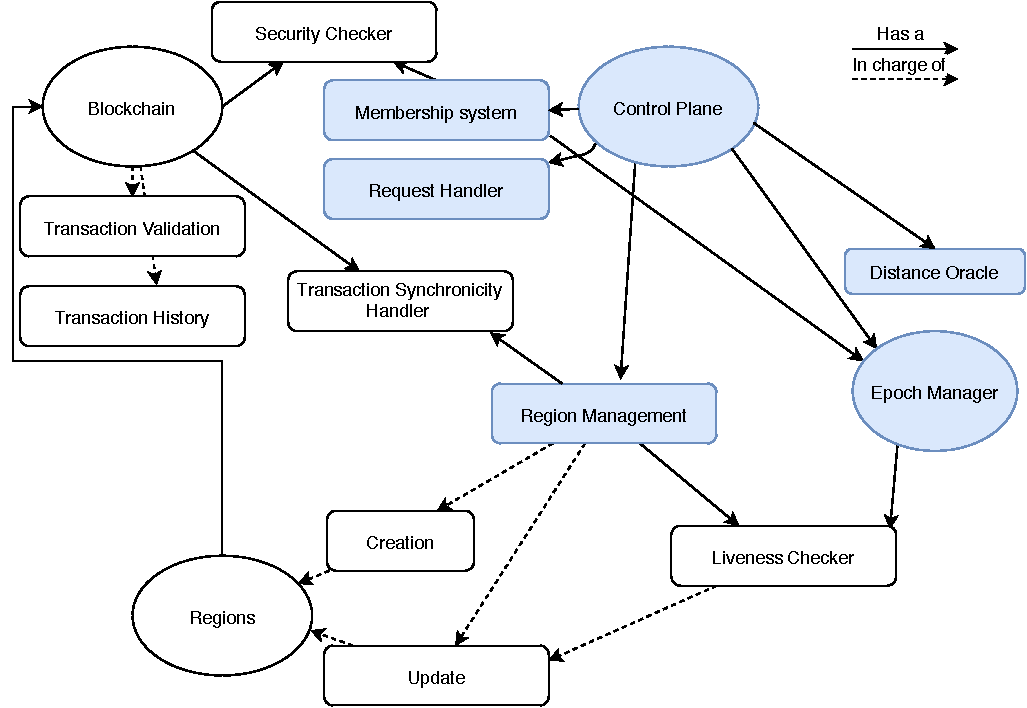
\includegraphics[width=400pt]{figures/Nyle_components} \caption{List of modules
of Nyle} \label{fig:modules} \end{figure}


\subsection{Membership Component}

At each epoch, a registry contract containing a summary of all participants is
created. Registration use endorsement (for example solution to a proof-of-work
problem).  This system will be global. Nodes can ask the participants of the
system to know the identity of other nodes. To validate a new contract  it
should be signed by the majority of the nodes of the previous epochs.

\subsection{Locality Component}

 The role of the locality component is to give all pairwise latencies between
 nodes of the system. We assume it already exists (distance oracle), or it can
 be computed by nodes. In the first model all pairwise latencies is computed
 between each node and every node agree on them via consensus. 
 
 \subsection{Region Component} This component is used to create and update
 regions. For the simple case, this part will be based on CRUX. At each epoch
 CRUX is run based on the new registration, and region are created.
 
 \subsection{Epoch Component} The epoch manager is linked to the membership
 system (we allow to change membership at the beginning of one epoch). New
 nodes can join at the beginning of one epoch. If nodes have moved, the region
 component will change or maintain their assignment at the beginning of one
 epoch. 

Epochs happen at a defined rhythm (e.g. one day). This frequency can be
shortened to ensure that nodes that want to join do not wait too long, or made
longer if one wants regions not to be redrawn too frequently. 

\subsection{Request Handler} The control plane is the right part to get
requests as it is aware of the nodes location and region assignment. It will be
in charge of answering the request for nodes assignment and nodes location. 

\begin{figure}[!h] \centering
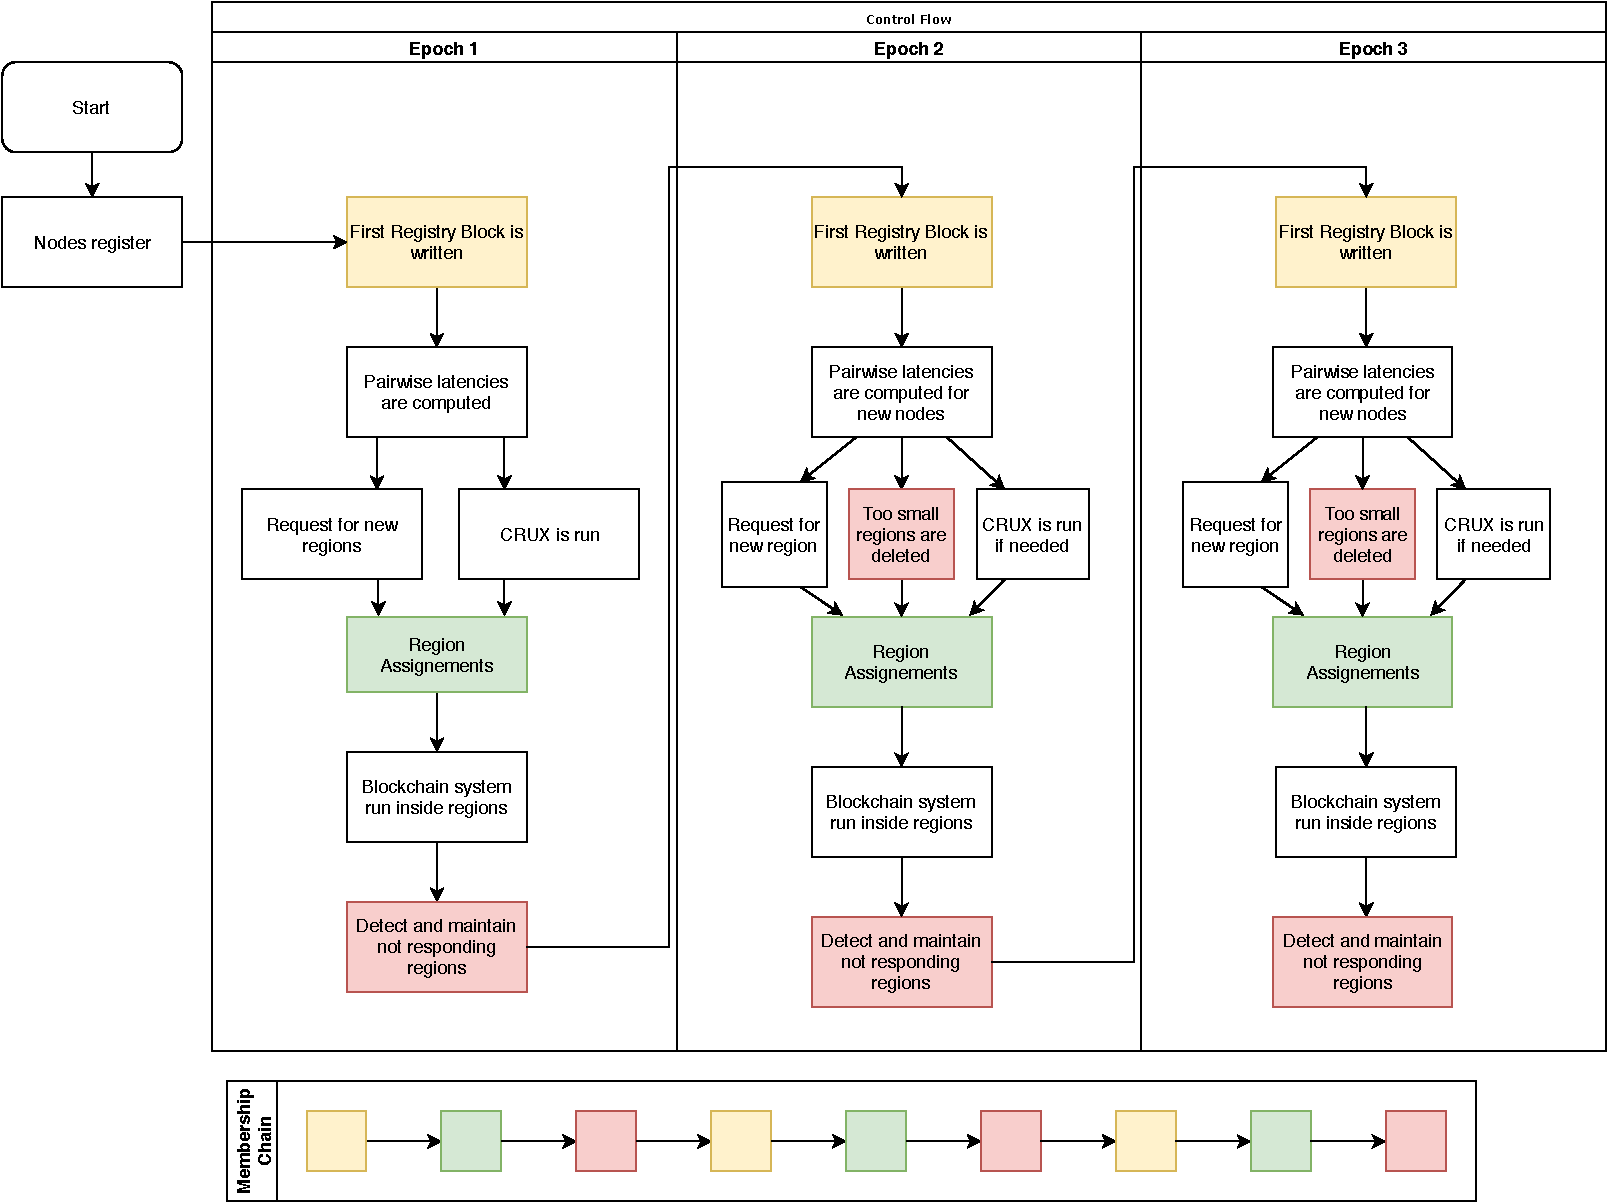
\includegraphics[width=400pt]{figures/Nyle_controlflow} \caption{General control Flow
of Nyle} \label{fig:modules} \end{figure}

\section{First version : Simple Control plane}
This version presents the first version of the Control Plane. In which most of the work is done on the membership component. At each epoch nodes can join if they manage to get an approval from the member of the previous region. The locality component in this model is brute force : every node computes its pings to every other nodes and consencus is made on that information. The region component in this model is really simple : based on the registration, and the pings, CRUX is run at each epoch. Redrawing the map of the entire system. 




\subsection{Membership Protocol}



%%%%%%%%%%%%%%%%%%%%%%%%
\chapter{Implementation}
%%%%%%%%%%%%%%%%%%%%%%%%

The implementation covers some of the implementation details of your project.
This is not intended to be a low level description of every line of code that
you wrote but covers the implementation aspects of the projects.

This section is usually 3-5 pages.


%%%%%%%%%%%%%%%%%%%%
\chapter{Evaluation}
%%%%%%%%%%%%%%%%%%%%

In the evaluation you convince the reader that your design works as intended.
Describe the evaluation setup, the designed experiments, and how the
experiments showcase the individual points you want to prove.

This section is usually 5-10 pages.


%%%%%%%%%%%%%%%%%%%%%%
\chapter{Related Work}
%%%%%%%%%%%%%%%%%%%%%%

The related work section covers closely related work. Here you can highlight
the related work, how it solved the problem, and why it solved a different
problem.  Do not play down the importance of related work, all of these systems
have been published and evaluated! Say what is different and how you overcome
some of the weaknesses of related work by discussing the trade-offs. Stay
positive!

This section is usually 3-5 pages.


%%%%%%%%%%%%%%%%%%%%
\chapter{Conclusion}
%%%%%%%%%%%%%%%%%%%%

In the conclusion you repeat the main result and finalize the discussion of
your project. Mention the core results and why as well as how your system
advances the status quo.

\cleardoublepage \phantomsection \addcontentsline{toc}{chapter}{Bibliography}
\printbibliography

% Appendices are optional \appendix %%%%%%%%%%%%%%%%%%%%%%%%%%%%%%%%%%%%%%
% \chapter{How to make a transmogrifier} %%%%%%%%%%%%%%%%%%%%%%%%%%%%%%%%%%%%%%
%
% In case you ever need an (optional) appendix.
%
% You need the following items: \begin{itemize} \item A box \item Crayons \item
% A self-aware 5-year old \end{itemize}

\end{document}
